\chapter{Abschlussaufgabe OAR}
OAR ist ein opensource Batchsystem. Es findet vorallem Anwendung im HPC Bereich,
Dass OAR bereit ist produktiv eingesetzt zu werden, beweist seine Benutzung in Projekten wie Grid'5000.
\begin{figure}[H]
	\centering
	\includegraphics[scale=1.5]{grid5000.jpg} 
	\vspace{-10pt}
	\caption{Grid'5000}
\end{figure}
Zuerst wird die zugrundeliegende Architektur erklärt und die dazugehörigen Installationsschritte auf dem Debiansystem beschrieben,
da diese nicht trivial sind.
Anschließend werden Unterschiede zum Batchsystem Slurm verdeutlich.
Zuletzt werden noch Benchmarks beider Batchsysteme gezeigt und verglichen.\pagebreak
\section{Architekur}
Eine typische OAR Installation besteht aus vier Komponenten. All diese sind im Debian Repository in der (aktuellen) Version 2.5.4-2 
zu finden:
    \begin{itemize}
        \item{Server node}
        \item{Frontend node}
        \item{Computing node}
        \item{Optional: Visualisierungsserver}
    \end{itemize}
    Debian Pakete:
    \begin{itemize}
        \item{oar-server}
        \item{oar-user}
        \item{oar-node}
    \end{itemize}

    \begin{figure}[h]
    \centering
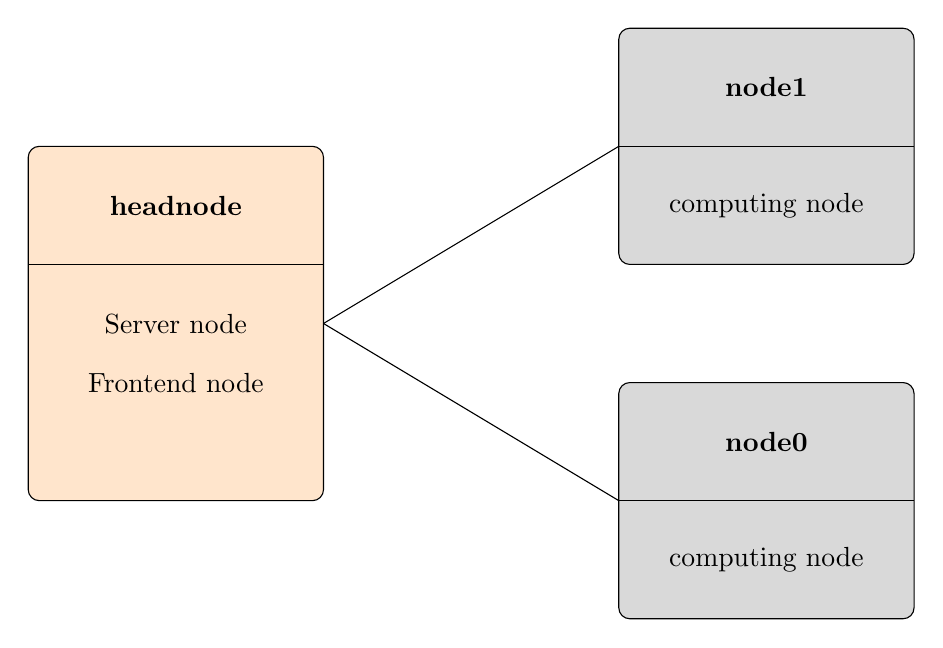
\begin{tikzpicture}[scale=1.5]
        %headnode
        \draw [rounded corners,fill=orange!20](0,1) rectangle (2.5,4); 
        \node at (1.25,3.5)[font=\bfseries] {headnode};
        \draw (0,3) -- (2.5,3);
        \node at (1.25,2.5) {Server node};
        \node at (1.25,2) {Frontend node};
        %node0
        \draw [rounded corners,fill=gray!30](5,0) rectangle (7.5,2); 
        \node at (6.25,1.5)[font=\bfseries] {node0};
        \draw (5,1) -- (7.5,1);
        \node at (6.25,0.5) {computing node};
        %node1
        \draw [rounded corners,fill=gray!30](5,3) rectangle (7.5,5); 
        \node at (6.25,4.5)[font=\bfseries] {node1};
        \draw (5,4) -- (7.5,4);
        \node at (6.25,3.5) {computing node};
        %edges
        \draw (2.5,2.5) -- (5,1);
        \draw (2.5,2.5) -- (5,4);
    \end{tikzpicture}
    \caption{Architekturskizze von OAR auf LCTP G1 Cluster} 
\end{figure}
\newpage

\section{Installation und Konfiguration}
    Auf den computenodes:
    \begin{lstlisting}[style=Bash]
    # apt-get install oar-node
	\end{lstlisting}
    Die /etc/sshd.conf auf den computenodes muss angepasst werden.
    Dieser Schritt ist in der Dokumentation auf der OAR Webseite nicht zu finden, wird aber benötigt.
    \begin{lstlisting}[style=Bash]
    AcceptEnv OAR_CPUSET OAR_JOB_USER
    PermitUserEnvironment yes
	\end{lstlisting}
    Auf dem headnode:
    \begin{lstlisting}[style=Bash]
    # apt-get install oar-server oar-server-mysql
    # oar-database --create --db-admin-user <user> -db-admin-pass <passwd>
    add nodes:
    # oarnodesetting -a -h node0
    # oarnodesetting -a -h node1
	\end{lstlisting}
	\newpage
\section{Benchmark}
	Zum Benchmarking wurden die Zeit gemessen, die das jeweilige Batchsystem benötigt
    einen Job in die Queue einzureihen, in Abhängigkeit der ANzahl schon wartender Jobs.\\
	\begin{figure}[H] \centering
		\includegraphics[scale=0.8]{../oar/output/pics/slurm.png} 
		\caption{Speedup[B3]}
	\end{figure}
	\newpage

	\begin{figure}[H]
		\centering
		\includegraphics[scale=0.8]{../oar/output/pics/oar.png} 
		\caption{Laufzeit Benchmark[B4]}
	\end{figure}
    \newpage 

	\begin{figure}[H]
		\centering
		\includegraphics[scale=0.8]{../oar/output/pics/oar_slurm.png} 
		\caption{Laufzeit Benchmark[B4]}
	\end{figure}
    \newpage 


	Ein Taurus Knoten hat jeweils zwei 8 Core Prozessoren auf einem Board. Daher zeigt sich bei 8 und 16 Cores eine Verschlechterung. 
	Ab 16 Cores läuft die Kommunikation zusätzlich über das Netzwerk.\\
	Ab 128 Cores ist bei 5.000 Punkten kein Speedup mehr vorhanden. Bei einer größeren Anzahl an Cores verschlechtert sich sogar die Laufzeit. Hier
	überwiegt der Overhead der MPI Kommunikation und das Zusammenführen der berechneten Cluster.\\
	\newpage
\section{Fazit}
	Es existieren viele Möglichkeiten zur Optimierung des parallelen Algorithmus. Zum Beispiel eine dynamische Verteilung der Punkte oder eine dynamische Anpassung
	der Wichtung um die Anzahl der benötigten Mean Shifts zu verringern.\\
	Die Kerngröße muss momentan noch manuell angegeben werden. Dies könnte auch automatisiert werden.\\
	Die markierten Cluster stimmen weitestgehend mit einer intuitiven Markierung überein. Punkte an der Grenze zu zwei Clustern werden jedoch häufig einem 
	dritten Cluster zugeordent (Birch3, (300k,300k)). Hier wäre eine Glättung möglich, in der Cluster mit wenigen Punkten in anliegenden Cluster aufgeteilt werden.\\
	\begin{figure}[H]
		\centering
		\includegraphics[scale=0.6]{../meanshift/output/pics/s4_colored.png} 
		\caption{S4, 5.000 Punkte[B5]}
	\end{figure}
\begin{thebibliography}{999}
	    \bibitem [0] {} Oar Official Website \url{https://oar.imag.fr}
	    \bibitem [1] {} Oar Universitys of Luxemburg \url{https://hpc.uni.lu/users/docs/oar.html}
	    \bibitem [2] {} Grid5000 Official Website \url{https://www.grid5000.fr}
	    \bibitem [3] {} Slurm Official Website \url{https://computing.llnl.gov/linux/slurm/}
	\newline
\end{thebibliography}
